\documentclass{article}
\usepackage{tikz}
\usetikzlibrary{shapes.geometric, arrows.meta, positioning}

\tikzstyle{startstop} = [rectangle, rounded corners, minimum width=3cm, minimum height=1cm, text centered, draw=black, fill=red!30]
\tikzstyle{process} = [rectangle, minimum width=3cm, minimum height=1cm, text centered, draw=black, fill=orange!30]
\tikzstyle{decision} = [diamond, minimum width=3cm, minimum height=1cm, text centered, draw=black, fill=green!30]
\tikzstyle{arrow} = [thick,->,>=stealth]

\begin{document}

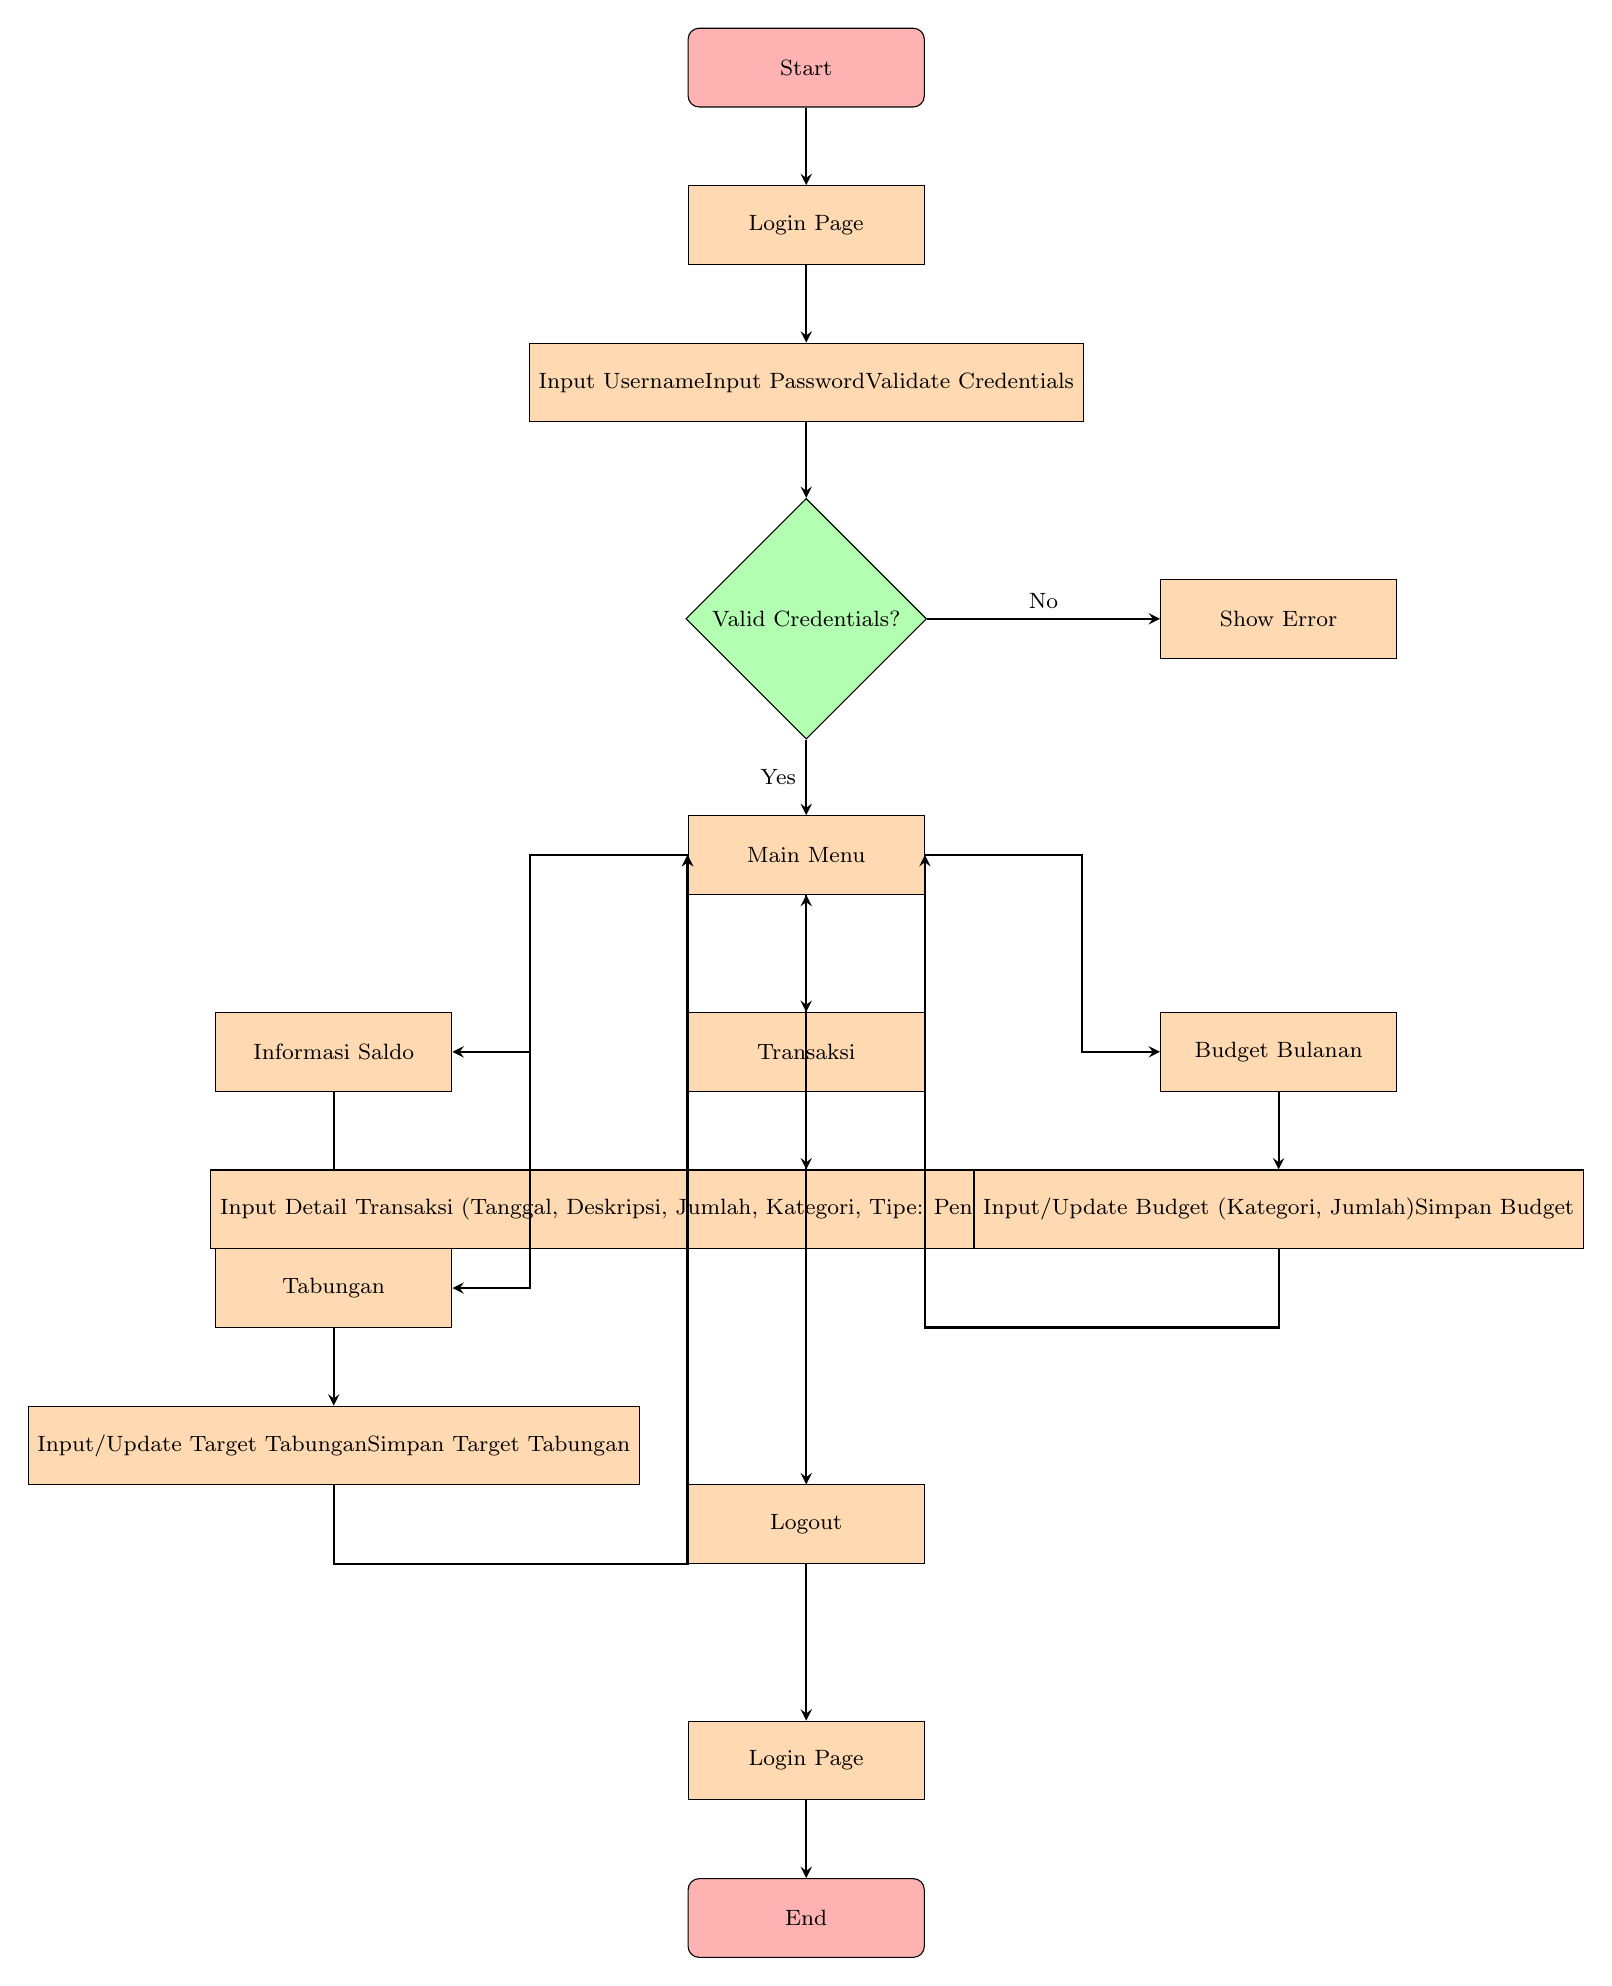
\begin{tikzpicture}[node distance=2cm, every node/.style={fill=white, font=\footnotesize}]

\node (start) [startstop] {Start};
\node (login) [process, below of=start] {Login Page};
\node (validate) [process, below of=login] {Input Username\\Input Password\\Validate Credentials};
\node (decision) [decision, below of=validate, yshift=-1cm] {Valid Credentials?};
\node (mainmenu) [process, below of=decision, yshift=-1cm] {Main Menu};
\node (error) [process, right of=decision, xshift=4cm] {Show Error};

\node (transaksi) [process, below of=mainmenu, yshift=-0.5cm] {Transaksi};
\node (detailtransaksi) [process, below of=transaksi] {Input Detail Transaksi (Tanggal, Deskripsi, Jumlah, Kategori, Tipe: Pengeluaran/Pemasukkan)\\Simpan Transaksi};

\node (budget) [process, right of=transaksi, xshift=4cm] {Budget Bulanan};
\node (inputbudget) [process, below of=budget] {Input/Update Budget (Kategori, Jumlah)\\Simpan Budget};

\node (saldo) [process, left of=transaksi, xshift=-4cm] {Informasi Saldo};

\node (tabungan) [process, below of=saldo, yshift=-1cm] {Tabungan};
\node (inputtabungan) [process, below of=tabungan] {Input/Update Target Tabungan\\Simpan Target Tabungan};

\node (logout) [process, below of=detailtransaksi, yshift=-2cm] {Logout};
\node (loginpage) [process, below of=logout, yshift=-1cm] {Login Page};
\node (end) [startstop, below of=loginpage] {End};

\draw [arrow] (start) -- (login);
\draw [arrow] (login) -- (validate);
\draw [arrow] (validate) -- (decision);
\draw [arrow] (decision) -- node[anchor=east] {Yes} (mainmenu);
\draw [arrow] (decision) -- node[anchor=south] {No} (error);

\draw [arrow] (mainmenu) -- ++(0,-1) -| (transaksi);
\draw [arrow] (transaksi) -- (detailtransaksi);
\draw [arrow] (detailtransaksi) -- ++(0,-1.5) -| (mainmenu);

\draw [arrow] (mainmenu.east) -- ++(2,0) |- (budget);
\draw [arrow] (budget) -- (inputbudget);
\draw [arrow] (inputbudget) -- ++(0,-1.5) -| (mainmenu.east);

\draw [arrow] (mainmenu.west) -- ++(-2,0) |- (saldo);
\draw [arrow] (saldo) -- ++(0,-1.5) -| (mainmenu.west);

\draw [arrow] (mainmenu.west) -- ++(-2,0) |- (tabungan);
\draw [arrow] (tabungan) -- (inputtabungan);
\draw [arrow] (inputtabungan) -- ++(0,-1.5) -| (mainmenu.west);

\draw [arrow] (mainmenu) -- ++(0,-5) -| (logout);
\draw [arrow] (logout) -- (loginpage);
\draw [arrow] (loginpage) -- (end);

\end{tikzpicture}

\end{document}
